\section{Contextualização do Problema e Justificativa}

O presente estudo tem como objetivo analisar a existência de vieses de julgamento na população geral e como esses vieses influenciam as escolhas políticas e econômicas. A pesquisa parte da premissa de que as crenças econômicas dos eleitores são frequentemente enviesadas, resultando em decisões políticas potencialmente sub-ótimas para o desenvolvimento econômico e social.

Além disso, é fundamental examinar a interação entre o Estado e a sociedade civil, considerando como essa dinâmica pode influenciar os vieses de julgamento. A relação entre a autoridade estatal e a capacidade de auto-organização da sociedade pode criar um ambiente que exacerba ou mitiga esses vieses. Nesse sentido, o equilíbrio entre a autoridade estatal e a liberdade individual é crucial para a formação das crenças e decisões políticas e econômicas dos cidadãos \cite{acemoglu2019narrow}.

Ademais, as teorias econômicas e a disseminação de conhecimento econômico desempenham um papel significativo na formação das crenças dos eleitores. A complexidade do pensamento econômico e as dificuldades na transmissão acessível dessas ideias ao público geral podem resultar em interpretações enviesadas que afetam diretamente as escolhas eleitorais e políticas. Neste contexto, as ideias de Bryan Caplan sobre o irracionalismo dos eleitores destacam como as preferências sistematicamente enviesadas podem distorcer o processo democrático e as políticas públicas \cite{The_Myth_of_the_Rational_Voter}.

Assim, este estudo não apenas investiga a presença de vieses de julgamento, mas também explora a interseção entre fatores históricos, sociais e econômicos que contribuem para a formação dessas crenças. Ao compreender essas interações complexas, podemos obter insights valiosos sobre como melhorar a educação econômica e promover decisões políticas mais informadas e eficazes, visando o progresso econômico e social.

Além disso, este trabalho contribui para o enriquecimento de uma nova área de estudo denominada "economia política comportamental". Essa área de pesquisa emergente busca integrar princípios da economia, ciência política e psicologia comportamental para entender melhor como os indivíduos tomam decisões econômicas e políticas e como esses processos podem ser influenciados por diversos fatores contextuais e cognitivos.

O método usado para a análise do presente trabalho será de revisão bibliográfica de várias fontes e análises empíricas já realizadas. A análise dos vieses de julgamento será feita a partir de uma abordagem interdisciplinar, considerando insights da economia comportamental, ciência política e história econômica. A pesquisa buscará identificar padrões e tendências nos vieses de julgamento e suas implicações para a democracia e as políticas públicas.

\section{Fundamentos Teóricos e Evidências Empíricas}

A análise dos fundamentos teóricos e das evidências empíricas na economia política comportamental é crucial para entender como os indivíduos tomam decisões econômicas e políticas. A economia comportamental, ao integrar conceitos da psicologia, desafia a noção tradicional de que os agentes econômicos são perfeitamente racionais e maximizadores de utilidade. Este campo de estudo examina como fatores cognitivos, emocionais e sociais influenciam as escolhas individuais e coletivas, oferecendo uma visão mais realista do comportamento humano.

Pesquisas têm demonstrado que as decisões dos eleitores e formuladores de políticas são frequentemente influenciadas por vieses cognitivos e heurísticas, que podem levar a escolhas sub-ótimas tanto no contexto econômico quanto no político. Esses vieses são moldados por diversos fatores, incluindo experiências passadas, influências culturais e a estrutura institucional na qual os indivíduos estão inseridos \cite{The_Myth_of_the_Rational_Voter, Systematically_Biased_Beliefs_about_Economics, saee1996}. 

A economia política comportamental emergiu como uma área de estudo promissora que busca entender essas dinâmicas complexas. Ao combinar insights da economia comportamental e da ciência política, essa disciplina oferece ferramentas valiosas para analisar como as crenças e atitudes dos eleitores impactam o funcionamento das democracias e a implementação de políticas públicas.


\subsection{O pensamento de economista} 
% o que caracteriza o pensamento de economista segundo a literatura, abordando a racionalidade, a busca por eficiência e a importância da informação.
% como o pensamento do economista se difere das percepções comuns da população comum.

Os economistas no geral operam sob o pressuposto de que os agentes econômicos são racionais e buscam maximizar sua utilidade ou satisfação a partir das escolhas disponíveis, o famoso "Homo Economicus". Esta abordagem implica que os indivíduos tomam decisões de forma lógica e consistente, com base nas informações disponíveis e a partir de uma avaliação cuidadosa das alternativas. É crucial também destacar a importância do pensamento da racionalidade das decisões econômicas, onde se argumenta que o comportamento racional é essencial para a eficiência e a eficácia das políticas econômicas \cite{Hausman_McPherson_Satz_2016}.

A análise de custo-benefício é uma ferramenta central no pensamento dos economistas. Ela permite a avaliação das opções de decisão com base nos custos e benefícios associados, assegurando que as decisões sejam eficientes e justas \cite{KenBinmore2008}. Os economistas utilizam essa abordagem para formular políticas que maximizem o bem-estar social, equilibrando os custos e benefícios de cada intervenção.


A informação desempenha um papel crucial nas decisões econômicas. Economistas acreditam que decisões de alta qualidade dependem da disponibilidade e do uso eficaz da informação, argumentando que a coleta, a análise e a disseminação de dados são fundamentais para o funcionamento eficiente dos mercados e das políticas públicas \cite{positive_economics_friedman}. Desde os anos 30, Friedrich Hayek tem destacado a importância da alocação do conhecimento na sociedade. Em seu artigo seminal de 1945, Hayek argumentou que o principal problema econômico enfrentado pela sociedade não é a alocação de recursos dados entre fins concorrentes, mas sim como assegurar o melhor uso dos recursos conhecidos por qualquer membro da sociedade, para fins cuja importância relativa apenas esses indivíduos conhecem \cite{hayek_knowledge_use}. Ele também enfatizou que a dispersão e a imperfeição de todo o conhecimento são fatos básicos com os quais as ciências sociais devem começar \cite{hayek_knowledge_dispersion}. No entanto, as limitações cognitivas dos indivíduos e a quantidade limitada de informação disponível podem levar a decisões sub-ótimas, conforme destacado por Daniel Kahneman em sua obra sobre heurísticas e vieses \cite{Judgment_under_Uncertainty}.

O pensamento econômico difere significativamente das percepções comuns da população. Enquanto os economistas enfatizam a racionalidade, a análise de custo-benefício e a importância da informação, a população frequentemente baseia suas decisões em heurísticas e vieses. Essas heurísticas são regras simples e intuitivas que as pessoas usam para tomar decisões rápidas e, embora úteis em muitos contextos, podem levar a erros sistemáticos \cite{Judgment_under_Uncertainty}. A população também é influenciada por crenças infundadas e emoções, o que pode resultar em decisões que não são necessariamente racionais ou eficientes do ponto de vista econômico \cite{thaler2016misbehaving}.

Em resumo, a abordagem de Gary Becker define o que hoje temos por regra atualmente:

\begin{citacao}
    \textit{Acho difícil acreditar que a maioria dos eleitores seja sistematicamente enganada quanto aos efeitos de políticas como a de quotas e tarifas de importações que persistem há tempos. Prefiro supor que o eleitor tem expectativas não enviesadas, ao menos, quanto a essas políticas persistentes. Eles talvez superestimem o peso-morto de algumas medidas e subestimem o de outras, mas, em média, eles tem uma ideia correta.
    } \newline \cite{becker1976}
\end{citacao}

\subsection{Economistas e os Vieses de Julgamento nos Eleitores}
% Fazer uma introdução igual Caplan faz no livro dele, falando sobre a importância da democracia e como ela depende de eleitores bem informados e racionais.

A democracia se fundamenta na ideia de que eleitores informados e racionais são capazes de tomar decisões que promovem o bem-estar coletivo e o desenvolvimento sustentável. Em "The Myth of the Rational Voter", Caplan argumenta que a eficácia da democracia depende criticamente da capacidade dos eleitores de avaliar políticas e candidatos de maneira objetiva e informada. Contudo, na prática, muitos eleitores sofrem de vieses de julgamento que distorcem suas percepções e decisões, resultando em escolhas que podem ser prejudiciais para a sociedade como um todo \cite{The_Myth_of_the_Rational_Voter}.

Acemoglu e Robinson, em "The Narrow Corridor", enfatizam que o engajamento político ativo e informado da população é crucial para manter o equilíbrio entre a autoridade estatal e a liberdade individual. Eles argumentam que a capacidade da sociedade de se organizar e participar ativamente nos processos políticos é fundamental para evitar a tirania e promover políticas que refletem verdadeiramente as necessidades e interesses da população \cite{acemoglu2019narrow}.

No entanto, os vieses de julgamento nos eleitores podem comprometer esse ideal democrático. Esses vieses são frequentemente resultado de heurísticas cognitivas, que são atalhos mentais usados para simplificar a tomada de decisão, mas que podem levar a erros sistemáticos. Entre os principais vieses que afetam os eleitores estão:

\begin{enumerate}
    \item Viés antimercado
    \item Viés antiestrangeiro
    \item Viés antitrabalho
    \item Viés pessimista
\end{enumerate}

Essa lista provém de uma análise de Caplan, que argumenta que esses vieses são comuns entre os eleitores e podem resultar em políticas públicas ineficazes e prejudiciais. Ele destaca que a educação econômica e a disseminação de conhecimento são essenciais para combater esses vieses e promover decisões políticas mais informadas e eficazes \cite{The_Myth_of_the_Rational_Voter}.

Atualmente, o estudo da "Economia Política Comportamental" e seus vieses está sendo revitalizado. No entanto, é crucial lembrar que a história do pensamento econômico sempre foi marcada por discussões sobre esses temas e seus correlatos.

Muitos dos famosos economistas do passado, como Adam Smith e Fréderic Bastiat, eram obcecados pela moralidade e pelas crenças teimosas do povo quanto a economia, a sua insistente resistência  aos princípios básicos do custo de oportunidade e a vantagem comparativa \cite{hart2019bastiat,Wells2013,The_Myth_of_the_Rational_Voter}.

Parece que as os economistas tem se esquecido de que a economia é uma ciência social e que as pessoas são seres humanos, com crenças e valores que muitas vezes não se alinham com a lógica econômica. Questões que hoje são levantadas como novas, já foram a tempos levantadas por economistas como Bastiat, que em sua obra "O que se vê e o que não se vê" já discutia sobre a dificuldade de se perceber os custos ocultos das políticas públicas e como elas se comportam na subjetividade \cite{hart2019bastiat}.

Estudar mais a fundo esses vieses presentes nos eleitores, tendo como um grande aliado a história do pensamento econômico se faz mais necessário que nunca. Lembrando que o problema do tema não é que os economistas não tem nada a dizer sobre o assunto, mas sim que eles tem muito a dizer porém relutam a ir em público e arriscar a sua credibilidade científica. Se fosse possível superar essa relutância teríamos muito a dizer \cite{The_Myth_of_the_Rational_Voter}. Gustavo Franco pode elucidar essa parte como ninguém:

\begin{citacao}
    \textit{[...] Tenha claro, por favor, que não há problema nenhum em atacar a sabedoria estabelecida [...]. Mas não perca de vista que ir contra o senso comum é um esporte radical: há muito risco e, se você errar, vai acabar no hospital. Sempre é preciso provar o que você diz, e costuma ser difícil. [...] Muito cuidado ao atacar a sabedoria estabelecida, pois na maioria das vezes você estará errado. Lembre-se de que o conhecimento que você herda se estabeleceu do trabalho diligente de muitos como você e eu, depois de anos e anos de tentativa, erro e decantação. \newline
    }  \cite{franco2022cartas}
\end{citacao}

Então temos em nossas mãos um cenário muito otimista apenas de revelar o que os economistas já sabem. Poucos economistas contemporâneos se preocupam com a história do pensamento econômico, e isso é um erro, deixando muitas discussões importantes ignoradas ou esquecidas \cite{mark_history}. A história do pensamento econômico é uma disciplina que nos ajuda a entender como as ideias econômicas evoluíram ao longo do tempo e como elas moldaram a sociedade em que vivemos. Ela nos permite ver como as ideias econômicas foram influenciadas por eventos históricos, mudanças políticas e avanços tecnológicos, e como essas ideias continuam a influenciar o pensamento econômico contemporâneo.

Porém o foco aqui são os vieses que não podem ser ignorados, explicando eles com base em no que os economistas acreditam ser o certo ao longo da história documentada e em contraste o que a população no geral acredita. Provas formais dos vieses estarão mais a frente.


\subsubsection{Viés antimercado}
% Descreva como o viés antimercado leva os eleitores a desconfiarem das soluções de mercado, favorecendo intervenções estatais.

O viés antimercado pode ser resumido na tendência de subestimar os benefícios do mercado, de seus mecanismos de mercado e superestimar os custos associados a ele \cite{sowell2000basic,sowell2004applied,The_Myth_of_the_Rational_Voter}. 

O cidadão comum tende a acreditar que o mercado é ineficiente e injusto, tende a ter séria dúvidas de até onde pode confiar e contar com empresas lucrativas para gerar produtos socialmente benéficos. Se foca somente na motivação do lucro da empresa e é deixado de lado a parte da disciplina imposta pelo mercado, que faz com que empresas que não atendem as necessidades do consumidor sejam eliminadas do mercado. Os economistas no geral admitem que, a busca incessante pelo lucro aliada as falhas e imperfeições de mercado podem gerar resultados ruins, não-economistas veem a ganância bem sucedida como algo socialmente prejudicial por si só \cite{The_Myth_of_the_Rational_Voter}.

Shumpeter, em sua obra "Capitalismo, Socialismo e Democracia", define com perfeição esse viés:

\begin{citacao}
    \textit{O capitalismo é julgado por juízes que têm a sentença de morte preparada. Eles darão este veredito, não importa o que a defesa diga; a única coisa que a defesa pode fazer é provocar uma mudança na acusação. \newline
    }  \cite{schumpeter1976capitalism}
\end{citacao}

Essa visão de que o lucro é simplesmente uma forma de transferência, uma exploração e que o mercado é um jogo de soma zero, onde o ganho de um é a perda de outro, é um dos principais fatores que levam os eleitores a desconfiarem das soluções de mercado e a favorecerem intervenções estatais. Vale ressaltar que "transferência" no dialeto econômico é um termo que se refere a um movimento descompromissado de riqueza de um agente para outro, sem que haja um aumento na riqueza total da sociedade. Levando isso como base, podemos concluir que as pessoas tendem a ver os lucros como um presente para os mais ricos. Portanto, a não ser que o governo intervenha limitando os lucros como questão de bom senso, a riqueza não será redistribuída de forma justa e eficiente \cite{The_Myth_of_the_Rational_Voter}. Essa forma de pensar é exatamente o que Thomas Sowell chama de "raciocínio de estágio único", ou seja, considerar apenas as consequências imediatas e óbvias de uma medida, ignorando as consequências indiretas e menos óbvias \cite{sowell2004applied}.

É importante lembrar que o lucro não é uma esmola, mas sim um \textit{quid pro quo}: o lucro é a recompensa por atender as necessidades e desejos dos consumidores de forma eficiente e inovadora. O lucro é o sinal de que uma empresa está gerando valor para a sociedade, alocando os recursos de forma eficiente, e não um mecanismo de exploração. Essa é a lição básica que Adam Smith nos ensinou em "A Riqueza das Nações": a "mão invisível" do mercado, guiada pela busca do lucro, silenciosamente convence os empresários egoístas a servir o bem comum \cite{smith1776inquiry}.

Desde o início da história registrada também temos o lucro aparecendo de forma prejudicial, como o exemplo do lucro sobre o empréstimo de dinheiro, o juros, que era considerado pecaminoso e injusto. Desde a mesopotâmia até a igreja católica medieval, por exemplo, proibindo a cobrança de juros, considerando-a uma forma de exploração e usura \cite{tomasdeaquino_summa_78}. Eugen von Böhm-Bawerk consegue elucidar essa questão de forma clara em seu clássico "Capital e Juro":

\begin{citacao}
    \textit{O credor geralmente é rico e o devedor, pobre, e o primeiro parece um homem odioso que suga o pouco que o pobre tem na forma de juros e que pode aumentar ainda mais sua riqueza supérflua. Não é de se surpreender, contudo, que tanto a Antiguidade quanto a Idade Média Cristã viam com maus olhos os juros. 
    } \newline \cite{von2022capital}
\end{citacao}

Para encerrar esta parte mostrando a visão dos economistas, uma pessoa que ouça ou veja economistas discutindo questões como essa, como Krugman ou Stiglitz, pode ter a impressão de que a parte benéfica do mercado ainda é controversa ou não está acertada \cite{krugman2003great,stiglitz2003roaring,The_Myth_of_the_Rational_Voter}. Nesse ponto, é importante entender que os economistas não estão debatendo se os preços dão incentivos ou se há uma enorme conspiração para manter os preços altos. Eles estão simplesmente explicando como o mercado funciona. Quase todos os economistas reconhecem que o mercado é a melhor maneira de alocar recursos escassos e que a concorrência é a melhor maneira de garantir que os preços sejam justos e que os consumidores sejam protegidos; eles discordam apenas sobre o grau disso.

\subsubsection{Viés antiestrangeiro}
% Descreva como o viés antiestrangeiro leva os eleitores a desconfiarem de acordos comerciais e imigração, favorecendo políticas protecionistas e anti-imigração.

É sempre interessante começar a explicação de um tema começando com uma pergunta fundamental a ser respondida: Estrangeiros? Será que pe mesmo mutuamente benéfico comercializar com eles?

Uma frase de Alan Blinder pode começar a explicar o motivo dessa desconfiança:

\begin{citacao}
    \textit{
        Quando os empregos são escassos, o instinto de autopreservação ganha força e a tentação de culpar a concorrência estrangeira é irresistível. Não só nos Estados Unidos que a mentalidade protecionista ganhou peso. O fato de muitos economistas considerarem míope e um autoboicote o esforço de, por meio do protecionismo, salvar empregos não cabe aqui. Os legisladores estão aí para ganhar votos, não elogios de intelectuais.
     } \newline 
    \cite{blinder1987hard}
\end{citacao}

Para reforçar o discurso, nada melhor que o pai da economia moderna para também citar o que naquela época já era considerado reprovável:

\begin{citacao}
    \textit{
         De que vale a prudência na conduta de todas as famílias se a escassez pode ser enganada num grande reino? Se um país estrangeiro puder nos fornecer uma mercadoria por um preço mais baixo do que o nosso, melhor comprá-la com uma parte do produto da nossa indústria, empregando de forma a termos alguma vantagem.
    } \newline
    \cite{smith1776inquiry}
\end{citacao}

Os economistas criticam o viés antiestrangeiro porque ele não só está errada como também essa visão entra de conflito com a economia mais elementar ensinada nos primeiros meses de graduação. Os livros mais usados, como o de Mankiw, ensinam que o comércio é mutuamente benéfico, que a especialização e a troca aumentam a produtividade e o bem-estar de todos os envolvidos. Nas palavras dele, de seus dez princípios de economia, o número cinco é:

\begin{citacao}
    \textit{
        [...] É fácil se enganar, porém, ao pensar na competição entre países. O comércio entre os Estados Unidos e a China não é como uma competição esportiva, em que um lado ganha e o outro perde. De fato, o oposto é verdadeiro: o comércio entre dois países pode ser bom para ambas as partes.
    } \newline
    \cite{mankiw2020introducao}
\end{citacao}

A Lei das Vantagens Comparativas é o fenômeno que é descrito acima. Essa teoria, desenvolvida por David Ricardo, reforça ainda mais a importância do comércio internacional. Segundo Ricardo, mesmo que um país seja menos eficiente na produção de todos os bens em comparação a outro, ainda é vantajoso para ambos os países se especializarem na produção dos bens nos quais têm uma vantagem comparativa (ou seja, onde têm uma menor desvantagem relativa) e comercializarem entre si. Isso ocorre porque a especialização baseada nas vantagens comparativas maximiza a produção global e o bem-estar econômico \cite{ricardo1817principles}.

Além disso, políticas protecionistas frequentemente resultam em ineficiências econômicas e redução do bem-estar. O livre comércio permite que os países aproveitem suas vantagens comparativas, promovendo a eficiência e o crescimento econômico global \cite{bhagwati2003free}.

Outro exemplo de viés antiestrangeiro é a desconfiança em relação à imigração. Muitos eleitores acreditam que a imigração prejudica a economia local, aumenta a concorrência por empregos e recursos escassos e ameaça a identidade cultural. Os economistas de hoje reconhecem facilmente os benefícios da imigração. A troca de trabalho é praticamente a mesma que a troca de mercadorias. Especialização e a troca aumentam a produção e o bem-estar de todos os envolvidos. A imigração aumenta a força de trabalho, a produtividade e a inovação, impulsionando o crescimento econômico e a prosperidade.

Em resumo, o viés antiestrangeiro leva os eleitores a desconfiarem de acordos comerciais e imigração, favorecendo políticas protecionistas e anti-imigração. No entanto, os economistas argumentam que o comércio internacional e a imigração são benéficos para a economia, promovendo a eficiência, o crescimento econômico e o bem-estar global.

Para finalizar com uma citação bem humorada, nada melhor que a de Steven Landsburg explicando que o comércio internacional é como uma tecnologia:

\begin{citacao}
    \textit{
        Há duas tecnologias para a produção de carros nos Estados Unidos. Uma delas é a manufatura em Detroit e a outra é a agricultura em Iowa. Todos conhecem a primeira; deixe-me falar da segunda. Primeira você planta as sementes, que são a matéria-prima dos carros. Você espera alguns meses até o trigo crescer. Daí você colhe o trigo, põe em navios e coloca os navios para cruzarem o Oceano Pacífico. Depois de alguns meses, os navios aparecem com Toyotas dentro deles.
    } \newline
    \cite{landsburg2012armchair}
\end{citacao}


\subsubsection{Viés antitrabalho}
% Discuta como o viés antitrabalho leva a uma resistência às mudanças tecnológicas e inovações. 

\begin{citacao}
    \textit{
        Deveríamos desejar, claro, que cada hectare de terra produza pouco trigo e cada grão de trigo gere pouco sustento - em outras palavras, que nossas terras sejam estéreis. [...] Pode-se até dizer que as oportunidades de trabalho deveriam ser diretamente proporcionais a essa esterilidade. [...] O que deveríamos desejar ainda mais é que a inteligência humana seja debilitada ou extinta, já que, enquanto sobreviver, ela se põe a aumentar a proporção entre fins e meios e entre produção e esforço.
    } \newline
    \cite{bastiat1859sofismas}
\end{citacao}

Por que parece que esse trecho de texto incomoda tanto? Esse trecho foi retirado do livro "Sofismas Econômicos" de Bastiat, o livro é uma coletânea de ensaios nos quais Bastiat critica e desmonta diversos sofismas econômicos, ou seja, argumentos falaciosos que, embora aparentemente lógicos, levam a conclusões incorretas ou enganosas sobre economia.

O público geralmente acredita que é melhor gastar do que economizar trabalho. Essa visão de que o trabalho é uma virtude em si mesma, independentemente de sua produtividade ou eficiência, é um dos principais fatores que levam os eleitores a resistirem às mudanças tecnológicas e inovações. A visão de produção de mais bens consumidos em menos horas ser vista não como um como um progresso e sim como um perigo, é o cerne do viés antitrabalho, a tendência de subestimar os benefícios econômicos de conservar o trabalho \cite{The_Myth_of_the_Rational_Voter}.

A população no geral observa a destruição de empregos pela tecnologia como algo terrível e os economistas em contraste veem a essência do crescimento econômico - a produção de mais com menos \cite{Myths-of-Rich-and-Poor,krugman2015accidental,davis1996job,innocence_and_design,bastiat1995selected}. Alan Blinder explica:

\begin{citacao}
    \textit{
        Se você fizer a pergunta diretamente, "Uma maior produtividade é melhor do que uma menor produtividade?", poucas pessoas responderão negativamente. No entanto, mudanças nas políticas frequentemente são vendidas como formas de "criar empregos". Existem duas maneiras de criar empregos. A forma socialmente benéfica é aumentar o PIB, para que haja mais trabalho útil a ser feito. Mas também podemos criar empregos garantindo que cada trabalhador seja menos produtivo. Assim, será necessário mais trabalho para produzir a mesma quantidade de bens. Essa última forma de criação de empregos realmente aumenta o emprego; mas é o caminho para a pobreza, não para a riqueza.
    } \newline
    \cite{blinder1987hard}
\end{citacao}

Onde está a falha nesse pensamento? A falha está em não perceber que o trabalho é um meio, não um fim em si mesmo. O objetivo da economia é maximizar a produção e o bem-estar, não o esforço e a atividade. A inovação e a automação são essenciais para aumentar a produtividade, reduzir os custos e melhorar a qualidade de vida. A resistência às mudanças tecnológicas e inovações pode resultar em ineficiências econômicas e perda de oportunidades de crescimento.

Para o indivíduo prosperar, ele precisa apenas de seu emprego. No entanto para a sociedade prosperar, ela precisa de indivíduos fazendo seus trabalhos, inovação e produtividade. A inovação e a produtividade são os motores do crescimento econômico e do progresso social. 

Porém essa guerra travada não é atual, a séculos os economistas já diagnosticaram a sociedade com esse problema. Bastiat havia relatado isso em sua época e dizia que esse pensamento era um "sisifismo" e, referência ao mito grego de Sísifo. Ele explicava:

\begin{citacao}
    \textit{
        O esforço em si constitui e mede a riqueza. Progredir é aumentar a relação entre esforço e resultado. Seu ideal pode ser representado pelo trabalho de Sísifo, ao mesmo tempo estéril e eterno. \newline
        A riqueza aumenta proporcionalmente ao aumento da relação entre resultado e esforço. A perfeição absoluta, cujo arquétipo é Deus, consiste na maior distância possível entre esses dois termos, ou seja, uma situação em que nenhum esforço produz resultados infinitos.
    } \newline
    \cite{bastiat1859sofismas}
\end{citacao}

O bom senso diz as maquinas e tecnologias facilitam a vida do ser humano, porém o público diz o contrário chamando de ingenuidade, observando que a tecnologia destrói empregos. Será que essa segunda visão é realmente a correta e não temos realmente um progresso?

\begin{citacao}
    \textit{
        Em 1800, era necessário que quase 95 de cada 100 americanos trabalhassem na agricultura para alimentar o país. Em 1900, esse número caiu para 40. Hoje, são apenas 3. Os trabalhadores que não são mais necessários nas fazendas foram redirecionados para a produção de novas casas, móveis, roupas, computadores, produtos farmacêuticos, eletrodomésticos, assistência médica, filmes, aconselhamento financeiro, videogames, refeições gourmet e uma variedade quase vertiginosa de outros bens e serviços. O que temos em lugar das longas horas nos campos é a riqueza de bens e serviços que surgem ao permitir que o dinamismo econômico opere, onde e quando for necessário.
    } \newline
    \cite{Myths-of-Rich-and-Poor}
\end{citacao}

Podemos ver com base na citação que a economia se renova com uma turbulência interminável, transferindo recursos para onde eles são necessários, substituindo funções antigas por novas.

Esses tipos de argumentos parecem muito duros para o público no geral e provavelmente é por isso que são tão impopulares. Preferem se sentir solidários que pensar racionalmente. Esse sentimento no lugar da racionalidade é o que caracteriza os vieses em sí.

\subsubsection{Viés pessimista}
% Descreva como o viés pessimista faz com que os eleitores tenham uma visão negativa sobre a economia, mesmo em tempos de crescimento.

O público acredita que as condições econômicas não são tão boas quanto realmente são. Esse viés pessimista leva os eleitores a terem uma visão negativa sobre a economia, mesmo em tempos de crescimento. Eles veem o mundo de mal a pior, acreditando que a economia está em declínio, que a desigualdade está aumentando e que o futuro é sombrio, sem muito espaço para a esperança. Esse pensamento é o chamado viés pessimista, a tendência de subestimar o progresso econômico e social e superestimar os problemas e desafios do passado recente, atual e futuro \cite{The_Myth_of_the_Rational_Voter}.

Smith ridicularizava essa visão pessimista em sua obra "A Riqueza das Nações" dizendo que "há um bocado de ruína em uma nação" \cite{smith1776inquiry}. As economias de porte podem progredir, e geralmente o fazem, a pesar de seus desafios e intermináveis obstáculos. A história econômica é uma história de progresso, inovação e crescimento. No entanto, o viés pessimista leva os eleitores a subestimarem esses avanços e a se concentrarem nos problemas e desafios que ainda persistem, ficando com um pensamento que se resume sempre a estagnação versus declínio \cite{The_Myth_of_the_Rational_Voter}.

Um sinal clássico dessa retórica pode ser vista em vários lugares. Arthur Herman escreve que "Praticamente todas as culturas do passado ou presentes acreditam não ser dignas de seus antepassados" \cite{herman1997idea}. Arthur Lovejoy e George Boas também expressam que essa visão é quase universal:

\begin{citacao}
    \textit{
        Não é uma conjectura improvável que o sentimento de que a humanidade estava se tornando excessivamente civilizada, que a vida estava ficando muito complicada e refinada demais, data da época em que os homens das cavernas se tornaram tal. Não é difícil supor — se os homens das cavernas eram minimamente parecidos com seus descendentes — que entre eles não havia quem discursasse com desprezo sobre a covarde efeminação de viver sob abrigo ou sobre o exasperante inconveniente de constantemente retornar para comer e dormir no mesmo lugar, em vez de serem livres para vagar em amplos espaços abertos.
    } \newline
    \cite{lovejoy_boas_1965}
\end{citacao}

Apesar de não ser tão comum economistas analisarem esse sentimento pessimista, ele é muito presente na sociedade intelectual através dos séculos. David Hume, por exemplo, em sua obra "Ensaios Morais e Políticos" já discutia sobre a tendência de se ver o passado com uma visão mais positiva do que o presente e o futuro, e que isso era um erro. Ele dizia:

\begin{citacao}
    \textit{
        O humor de culpar o presente e admirar o passado está fortemente enraizado na natureza humana e exerce influência até mesmo sobre pessoas dotadas do julgamento mais profundo e do aprendizado mais extenso. \newline
        Quando os terrores reais estão ausentes, a alma, ativa em seu próprio prejuízo e alimentando sua inclinação predominante, encontra terrores imaginários, aos quais não impõe limites de poder e malevolência.
    } \newline
    \cite{Hume1875}
\end{citacao}

Como Hume cite, até mesmo "pessoas com um julgamento mais profundo e um aprendizado mais extenso" são afetadas por esse viés pessimista. No mundo dos grandes pensadores de economia temos exemplos de pessoas que não conseguem escapar desse viés. 

Karl Marx dizia:

\begin{citacao}
    \textit{
        O desenvolvimento da indústria moderna, portanto, elimina os próprios alicerces sobre os quais a burguesia produz e se apropria de produtos. O que a burguesia, portanto, produz, acima de tudo, são os seus próprios coveiros. A sua queda e a vitória do proletariado são igualmente inevitáveis.
    } \newline
    \cite{marx1988communist}
\end{citacao}

Shumpeter também não escapava desse viés, ele dizia:

\begin{citacao}
    \textit{
        O capitalismo pode sobreviver? Não. Não creio que possa... não é da tese de que não pode viver por causa da sua ineficiência econômica... mas é por causa do seu próprio sucesso, que levará à sua queda.
    } \newline
    \cite{schumpeter1976capitalism}
\end{citacao}

Como esse grandes níveis de pessimismo podem coexistir com o progresso econômico e social que temos visto ao longo da história? Gregg Easterbrook ridiculariza  a incapacidade dos cidadãos do mundo desenvolvido de apreciarem sua condição afortunada. Em seu livro "Progress Paradox" ele diz:

\begin{citacao}
    \textit{
        Nossos antepassados, que trabalharam e se sacrificaram incansavelmente na esperança de que seus descendentes um dia fossem livres, confortáveis, saudáveis e educados, ficariam desanimados ao observar como negamos amargamente que agora somos todas essas coisas.
    } \newline
    \cite{easterbrook2004progress}
\end{citacao}

Matt Ridley oferece uma visão contrastante ao viés pessimista ao argumentar que o progresso econômico e social é inevitável devido à combinação da inovação e da troca de ideias. Ridley destaca que, ao longo da história, a humanidade tem conseguido superar desafios e melhorar suas condições de vida através da colaboração e do comércio. Ele observa:

\begin{citacao}
    \textit{
        O mundo está melhorando, não piorando. A vida humana ficou mais longa, mais saudável, mais livre, mais sábia, mais informada e mais pacífica em apenas meio século. As coisas têm melhorado em todas as regiões do mundo.
    } \newline
    \cite{ridley2010rational}
\end{citacao}

Ridley enfatiza que a inovação tecnológica e a globalização têm desempenhado papéis cruciais na melhoria das condições de vida globais, contrariando o pessimismo comum. Ele argumenta que a natureza colaborativa do ser humano é a principal força motriz por trás do progresso contínuo e que, embora existam problemas e desafios, a tendência geral é de avanço e crescimento:

\begin{citacao}
    \textit{
        A inovação, ao contrário do que muitos pensam, não está se esgotando. Pelo contrário, está se acelerando, alimentada pela troca de ideias e pela colaboração global.
    } \newline
    \cite{ridley2010rational}
\end{citacao}

Dessa forma, Ridley sugere que a tendência humana de focar nos aspectos negativos e ignorar o progresso é um erro que pode ser corrigido através de uma perspectiva mais equilibrada e informada sobre a história e o desenvolvimento humano.

Finalizando a parte dos vieses, podemos ver que os economistas tem uma relação de amor e ódio com os vieses. Os vieses antimercado, antiestrangeiro, antitrabalho e pessimista são os mais evidentes e provavelmente existem muitos outros a serem descobertos. Na verdade muitos alunos de graduação em economia chegam nas aulas com eles. Os alunos não são uma tabula rasa para seus professores, eles já tem uma visão de mundo e muitas vezes essa visão é distorcida. O que os economistas podem fazer é tentar corrigir esses vieses, mostrando que o mercado é benéfico, que o comércio é mutuamente benéfico, que a inovação e a produtividade são essenciais para o crescimento econômico e que o progresso é inevitável. No entanto, como Gustavo Franco disse, é um esporte radical ir contra o senso comum, e se você errar, vai acabar no hospital. Sempre é preciso provar o que você diz, e costuma ser difícil.

\subsubsection{A influência dos vieses e a armadilha das ideias}
% Falar de como esses vieses se enquadram em um problema econômico? Falar da dinâmica proposta pela noção de que indivíduos podem ter preferências por crenças.

Depois de toda essa discussão sobre os vieses, podemos ver que eles são muito mais do que simples erros de julgamento. Eles são uma parte fundamental da natureza humana e desempenham um papel crucial na formação de nossas crenças e preferências. Os vieses são uma forma de heurística, ou regra prática, que nos ajuda a tomar decisões rápidas e eficientes em situações complexas e incertas. 

Mas porque, mesmo ao longo da história com tantos autores, das mais variadas áreas falando sobre eles, alertando sobre os perigos que eles podem causar, ainda assim eles persistem? A resposta que se tem no momento é que temos um preferência sobre crenças, ou seja, temos uma preferência por acreditar em coisas que nos fazem sentir bem, mesmo que não sejam verdadeiras. 

O problema principal dessa afirmação é que ela contraria a "abordagem da escolha racional" da Ciência Social Contemporânea, dizendo que trata a nossa história como uma "história sem tolos". Já aqui colocamos em uma diferente abordagem nos holofotes, a tolice, ou em termos técnicos, a irracionalidade.

Mas o que pode vir a ser essa irracionalidade? Os economistas no geral supõem que crenças são meios para um fim, e não o fim em sí. Porém, a ideia de que as crenças são um fim em sí mesmo é uma ideia que tem ganhado força nos últimos anos. A ideia de que as pessoas têm preferências por crenças, ou seja, que elas preferem acreditar em coisas que as fazem sentir bem, mesmo que não sejam verdadeiras, opiniões que gostamos de acreditar e as valorizamos por sí mesmas, e não por suas consequências. Shermer diz: "Sem alguma estrutura de crença, muitas pessoas não veem sentido neste mundo" \cite{shermer2002people}.

Falando em jargão econômico, as pessoas têm uma "demanda por crenças", ou seja, elas têm preferências sobre crenças. Deixar que sentimentos e uma ideologia corrompam nosso raciocínio é uma maneira de satisfazer essa demanda. Ayn Rand chama esse fenômeno de “blanking out”, ou seja, um "apagão": a interrupção intencional do pensamento, da consciência, a recusa em pensar; não a cegueira mas a recusa em ver; não a ignorância mas a recusa em saber.

Fora da economia, a ideia de que as pessoas preferem ter uma crença sobre outras é antiga. Em "O Ensaio Sobre o Entendimento Humano" de John Locke, ele fala de um "entusiasmo, no qual a razão é roubada". Para ele, ser um entusiasta é aceitar ideias dúbias com base na emoção:

\begin{citacao}
    \textit{
        Para que a evidência de que qualquer proposição é verdadeira (exceto aquelas que são autoevidentes) resida apenas nas provas que um homem tem dela, quaisquer graus de assentimento que ele conceda além dos graus dessa evidência, é claro que todo o excedente de certeza se deve a alguma outra afeição, e não ao amor pela verdade.
    } \newline
    \cite{locke2014ensaio}
\end{citacao}

Observe os dois componentes de sua citação. O primeiro é o “excedente de certeza”. Locke observa que as pessoas atribuem probabilidades às crenças maiores do que as evidências justificam. O segundo é “outras afeições”. A causa do excesso de confiança, na visão de Locke, é o conflito de motivos \cite{The_Myth_of_the_Rational_Voter}. 

Quando se fala também de preferências por crenças, é quase impossível não citar religiões. É o que Shermer dizia em ver sentido neste mundo. As pessoas querem que as respostas de suas religiões sejam verdadeiras, mesmo que não sejam. Elas se recusam a estudar, a procurar contraprovas e mesmo a refletir com a prova em seus colos. Elas querem acreditar, e acreditam. Lembrando que aqui não se está dizendo que a religião é falsa, mas sim que as pessoas  não procuram a verdade, mesmo que ela a seja. Preferem o dogma.

Lembrando do viés antiestrangeiro, as pessoas podem culpar os estrangeiros pelos problemas internos como uma fonte de consolo. Eles podem até mesmo reconhecer que o livre-comércio é benéfico, mas ainda resistem e ficam ressentidos quando lhes mostram as vantagens comparativas. O mesmo pode acontecer com o viés pessimista, a nostalgia traz as pessoas um conforto ao reviver memórias passadas, ignorando o progresso que foi feito.

Mas como a preferência sobre as crenças podem se conciliar com a Teoria da Escolha Racional? Uma pessoa que chegou muito perto dessa realização foi Anthony Downs em seu livro "Uma Teoria Econômica da Democracia". Ele conseguiu transformar a ignorância racional em elemento básico da Economia Política. Ele dizia que as pessoas não têm tempo para estudar todas as questões políticas, por que os retornos de ser bem-informado são muito baixos. Portanto, as pessoas têm incentivos para serem ignorantes sobre questões políticas \cite{downs1957economic}.

A lógica usada por ele pode ser resumida de maneira bem simples: tempo é dinheiro e adquirir informação exige tempo. Mas o que isso tem haver com a conciliação entre preferências por crenças e a Teoria da Escolha Racional? A resposta é que as pessoas têm incentivos para serem ignorantes sobre questões políticas, porque a informação é cara e os retornos são baixos. Mas isso ainda leva em conta a racionalidade, ou seja, as pessoas são racionais em sua ignorância. Porém o próprio Downs reconhece que a preferência sobre crenças existe, a irracionalidade:

\begin{citacao}
    \textit{
        Nosso desejo de evitar a irracionalidade política surge de (1) a complexidade do assunto, (2) sua incompatibilidade com nosso modelo de comportamento puramente racional, e (3) o fato de ser um fenômeno empírico que não pode ser tratado apenas com lógica dedutiva, mas também requer investigação empírica, que está além do escopo deste estudo.
    } \newline
    \cite{downs1957economic}
\end{citacao}

É impressionante saber que Downs tangenciou a irracionalidade política há 50 anos. Mas por que os economistas são tão hostis a ideia de estupidez, de irracionalidade ou mesmo da preferência por crenças? Uma resposta a essa pergunta pode ser de que qualquer erro popular, por mais estranho que este seja, parece confirmar a ignorância racional. Outra resposta é a mais básica, a de que faltam dados o bastante e ou não se consegue tirar proveito dos dados disponíveis para se fazer uma análise mais precisa. Aqui estamos indo além, onde Downs parou, estamos indo para a irracionalidade, para uma mentalidade de preferência por crenças.

Friedrich Hayek também abordou a limitação do conhecimento humano em decisões econômicas. Em seu famoso ensaio "O Uso do Conhecimento na Sociedade", Hayek argumentou que o conhecimento é disperso e fragmentado, o que dificulta a tomada de decisões centralizadas eficientes \cite{hayek_knowledge_use}. Segundo Hayek, a descentralização da tomada de decisão é crucial, pois permite que informações locais específicas sejam utilizadas de maneira mais eficaz. Ele também reconheceu que os agentes econômicos podem agir de maneira irracional devido às suas limitações cognitivas e à complexidade do ambiente em que operam.

A perspectiva de Hayek sobre a dispersão do conhecimento amplia a ideia de Downs sobre a ignorância racional. Enquanto Downs se concentra na racionalidade das escolhas de permanecer ignorante devido aos altos custos da informação, Hayek explica que mesmo que o indivíduo buscasse informações, ele ainda estaria limitado pela natureza fragmentada do conhecimento disponível na sociedade. Portanto, a preferência por crenças pode ser vista não apenas como uma escolha racional para evitar os custos da informação, mas também como uma consequência da impossibilidade de um único agente acessar e processar todo o conhecimento necessário para tomar decisões perfeitamente informadas.

E como isso se transforma em um problema econômico? A resposta é que as preferências por crenças podem levar a políticas públicas ineficientes e prejudiciais. Os eleitores podem votar com base em crenças irracionais, em vez de evidências e argumentos racionais. Eles podem apoiar políticas protecionistas, anti-imigração e intervencionistas, mesmo que essas políticas sejam prejudiciais para a economia e a sociedade. Eles podem resistir a mudanças tecnológicas e inovações, mesmo que essas mudanças sejam essenciais para o crescimento econômico e o progresso social. Eles podem ter uma visão negativa sobre a economia, mesmo em tempos de crescimento, e apoiar políticas que minam o progresso e a prosperidade.


\section{Evidências Empíricas}

Agora que já discutimos os vieses e a preferência por crenças, vamos ver como eles se manifestam na prática. Vamos analisar algumas evidências empíricas que mostram como os vieses afetam o comportamento dos eleitores e influenciam as políticas públicas.

\subsection{Estados Unidos da América}

Para o Estados Unidos é onde temos um maior rigor de evidências suportando a pesquisa \cite{The_Myth_of_the_Rational_Voter,Systematically_Biased_Beliefs_about_Economics,blendon-gap}. A análise dos vieses e preferências por crenças nos Estados Unidos é um campo com muitas pesquisas e estudos. Dentre esses estudos temos a SAEE, a Survey of Americans and Economists on the Economy, que é uma pesquisa que compara as opiniões dos americanos com as dos economistas sobre questões econômicas \cite{saee1996}.  

A análise desses vieses é suportada principalmente por Bryan Caplan e Robert Blendon em diversos artigos \cite{The_Myth_of_the_Rational_Voter,Systematically_Biased_Beliefs_about_Economics,think_like_economists,blendon-gap}. Caplan e Blendon argumentam que os eleitores americanos têm erros sistemáticos. Eles também argumenta que os eleitores têm uma preferência por crenças, ou seja, que eles preferem acreditar em coisas que os fazem sentir bem, mesmo que não sejam verdadeiras.

A SAEE tem como estrutura robusta de conjunto de dados sendo também a única que deliberadamente faz as mesmas perguntas a ambos os grupos sobre uma diversidade de tópicos. Os entrevistados foram 1.510 membros do público e 250 economistas com PhD; os primeiros foram selecionados aleatoriamente em todo o país a partir da população geral dos EUA, enquanto os últimos foram selecionados aleatoriamente entre os membros da AEA com PhD em economia, empregados em tempo integral como economistas e especializados em política econômica doméstica \cite{saee1996,Systematically_Biased_Beliefs_about_Economics,blendon-gap}. Os pesquisadores também coletaram informações detalhadas sobre as características pessoais de todos os entrevistados: renda familiar, nível de educação, raça, gênero, partido político, ideologia política, entre outros. 

Também é enfatizado o contraste marcante no SAEE entre as crenças dos economistas e do público. Eles também apresentam várias hipóteses possíveis para explicar as diferenças apresentadas:

\begin{itemize}
    \item As experiências dos indivíduos podem não refletir os dados oficiais.
    \item Quando as pessoas avaliam o desempenho da economia, as estatísticas do governo são apenas uma das várias fontes de informação que elas utilizam.
    \item Um grande número de americanos não acredita que as estatísticas econômicas do governo sejam precisas.
    \item A mídia tende a retratar a condição da economia como sendo pior do que realmente é, deixando o público excessivamente pessimista sobre a situação econômica do país.
    \item Os economistas são mais otimistas sobre o futuro econômico porque fazem parte de um segmento ocupacional, composto por profissionais e cientistas, que pode ter sido protegido em certa medida das consequências negativas das mudanças econômicas relatadas na pesquisa pela maior parte do público.
    \item Os americanos não possuem uma boa base de conhecimento sobre como a economia funciona e, portanto, podem ter dificuldade em fazer avaliações precisas sobre o desempenho da economia.
\end{itemize}

O restante do artigo vai se basear muito na SAEE, seja por seu conteúdo robusto ou por sua metodologia que é usada de inspiração para outras pesquisas.

Caplan faz um grande trabalho estatístico e empírico nas seções e conjuntos de perguntas da SAEE. Adicionalmente após este artigo, ele escreve um livro também com evidências da SAEE chamado "The Myth of the Rational Voter" \cite{The_Myth_of_the_Rational_Voter}.

As 37 perguntas principais da SAEE podem ser divididas em 4 partes. As duas primeiras partes podem ser usadas para explicar "por que a economia não está crescendo". Serão 18 questões sobre isso. As 7 questões da terceira parte podem ser usadas para dizer se algo é "bom", "ruim ou "neutro" para a economia. As 12 questões da quarta parte são perguntas diversas. É importante ressaltar que a SAEE tem mais de 37 questões, porém algumas perguntas não estavam presentes ambos grupos de entrevistados, e por isso não foram consideradas.

Há grandes lacunas de pensamento entre os economistas e o público. Por mais elitista que isso se apresente, é um fato e o padrão na literatura sobre preconceitos. Kahneman e Tvesky, por exemplo, descrevem o seu método como "a presença de um erro de julgamento que é demonstrado comparando as respostas com um fato consagrado [...]." \cite{Judgment_under_Uncertainty}. Mas consagrado por quem? Por especialistas, por pessoas que estudaram o assunto é claro.

Claro que existe a possibilidade de que os especialistas em geral estejam errados, afinal quem é que nunca errou? E além disso, se um físico, um matemático ou estatístico diz que o público está errado, é mais fácil de aceitar, afinal eles são especialistas em suas áreas. Mas por que a situação muda com um economista? Já dizia William Greider:

\begin{citacao}
    \textit{
        A democracia hoje está presa à mistica da elaboração de políticas "racionais", hipóteses rasas sobre o que constitui a prova política legítima. É uma barreira de privilégio porque ignora expressões políticas autênticas de cidadãos, exaltando os preconceitos e opiniões das elites.
    } \newline
    \cite{greider2010will}

\end{citacao}

Partindo deste ponto de vista, usar opiniões de "especialistas" em economia para impugnar as opiniões do público é um erro enorme. Mas de onde surge essa grande duvida de concordar com os economistas? Uma resposta pode surgir da grande incapacidade deles de simplesmente concordar. George Bernard Shaw dizia que "se todos os economistas fossem postos em fila, eles não chegariam a uma conclusão". Mas esse é um argumento muito raso e pode ser facilmente refutado. Uma outra hipótese é que os economistas sofrem de um viés específico chamado de "viés autoindulgente". Talvez por os economistas terem maior renda, empregos mais seguros, eles tendam a acreditar que o que é melhor para eles é melhor para o país. Marx ridicularizava essa ideia dizendo que "os economistas são os sacerdotes da burguesia" ou como defensores do capitalismo que os sugava \cite{marx_engels_capital}. Para ser equilibrado, Ludwig Von Mises também dizia algo parecido no entre-guerras da Alemanha:

\begin{citacao}
    \textit{
        Tudo o que os estudantes das ciências sociais aprenderam com seus professores foi que a economia é uma ciência espúria e que os chamados economistas são, como Marx disse, bajuladores apologistas dos interesses de classe injustos dos exploradores burgueses, prontos para vender o povo para os grandes negócios e o capital financeiro.
    } \newline
    \cite{mises_bureaucracy}

\end{citacao}

Porém ainda existe mais um viés que se torne possível de ser explorado, o viés de ideologia \cite{The_Myth_of_the_Rational_Voter}. A ideologia é um conjunto de crenças e valores que moldam a maneira como as pessoas veem o mundo e tomam decisões. A ideologia pode influenciar as preferências das pessoas por crenças, levando-as a acreditar em coisas que se alinham com suas visões políticas e morais, mesmo que não sejam verdadeiras. A ideologia pode ser um fator importante na formação de vieses e na tomada de decisões políticas \cite{The_Myth_of_the_Rational_Voter}.

Se formos apelar a esses dois vieses, o viés autoindulgente e o viés de ideologia, podemos ver que os criticos correm um risco. Tanto o viés autoindulgente quanto o viés de ideologia são, em principio, empiricamente comprováveis. Se é assim, então economistas ricos e leigos ricos pensam igual? E economistas conservadores e leigos conservadores pensam igual? 

Por que foi dado esta volta tão grande quando se estava apresentando a SAEE? A resposta é que a SAEE é um grande portfólio de respostas das mais variadas para testar essas hipóteses. Existem mensurações de todas as principais características sociais: renda familiar, estabilidade no emprego, raça, gênero, idade e até aumento de renda. Adicionalmente ela também tem duas medidas de ideologia.

Caplan também faz uma distinção adicional entre as pessoas, além de economistas e público geral. Ele faz a estimação do "público esclarecido", que seriam as pessoas que tem uma semelhança muito próxima nos dados com os economistas, com exceção de uma variável: o Phd em economia.

As questões serão divididas em três estatísticas:

\begin{enumerate}
    \item A crença média "bruta" do público em geral.
    \item A crença média "bruta" dos PhDs em economia.
    \item A crença média "estimada" do público esclarecido.
\end{enumerate}

Se a autoindulgência e a ideologia forem verdadeiras, então as respostas entre o público esclarecido e o publico geral devem ser muito próximas. Se a autoindulgência e a ideologia forem falsas, então as respostas entre o público esclarecido e os economistas devem ser muito próximas \cite{The_Myth_of_the_Rational_Voter}.

\subsubsection{Por que a economia não está crescendo?}

segundo caplan (\citeyear{The_Myth_of_the_Rational_Voter})

\begin{figure}[ht]
    \centering
    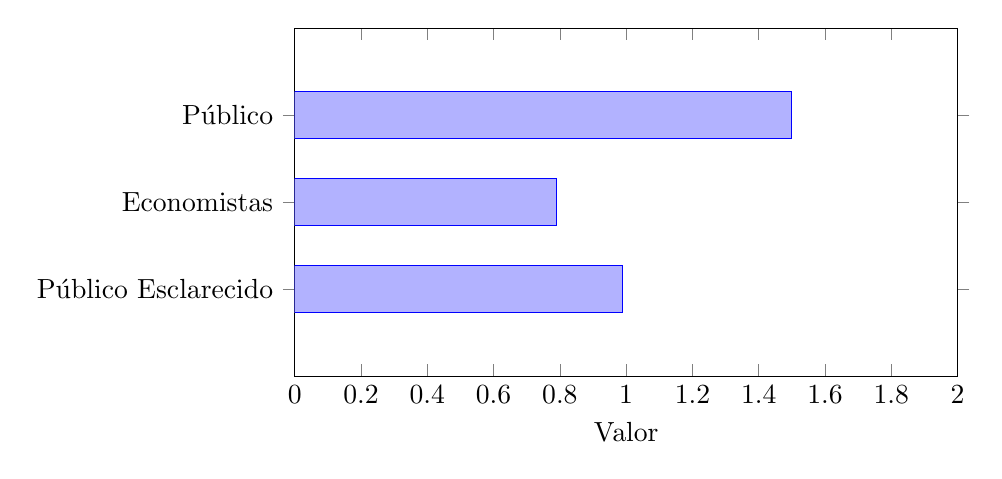
\begin{tikzpicture}
        \begin{axis}[
            xbar,
            symbolic y coords={Público, Economistas, Público Esclarecido},
            ytick=data,
            xmin=0, xmax=2,
            xlabel={Valor},
            bar width=0.6cm,
            width=10cm,
            height=6cm,
            enlarge y limits=0.5,
            y dir=reverse % Invert the y-axis to maintain the desired order
        ]
        \addplot coordinates {(1.5,Público) (0.79,Economistas) (0.99,Público Esclarecido)};
        \end{axis}
    \end{tikzpicture}
    \caption{Valores por grupo}
    \label{fig:valores_grupo}
\end{figure}


\subsection{Portugal}

\subsection{Brasil}


\section{Interpretação dos Resultados e Implicações}

\section{Conclusão}

